% Chapter Template

\chapter{Introduction} % Main chapter title

\label{Introduction}


\section{Problem}
Human pose estimation is a task based on a human's image or 3D points, and the model should locate the main joints in the human's body (head, neck, left and right arms, spin, etc.) as shown in the Figure  \ref{example}. Each joint is represented as a point in 2D or 3D space based on the task's objective.

\begin{figure}[htbp]
\centerline{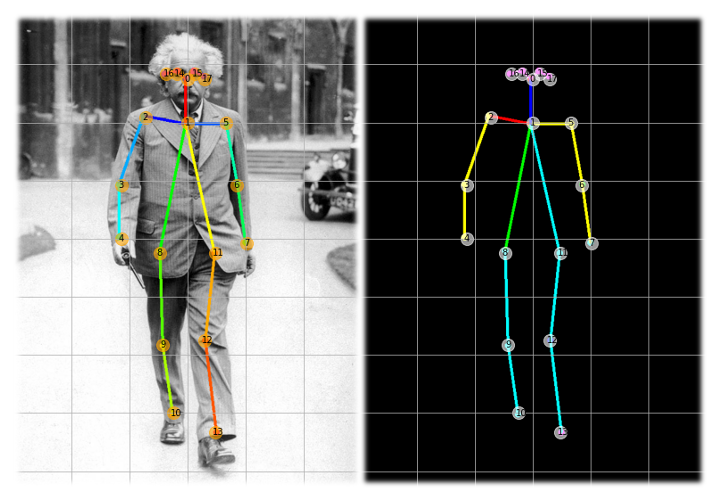
\includegraphics[scale=.5]{Figures/introduction-einstein.png}}
\caption{Example of human pose estimation key points \cite{rovai_realtime_2020}}
\label{example}
\end{figure}

A 3D point cloud is simply a set of points with three positional coordinates and represents points in 3D space. The points represent the shape of the object in 3D space. 3D point clouds are usually gathered by 3D scanners or dual-lens cameras.The output of scanners is point cloud where each point corresponds to some point on scanning surface with predefined precision. With the rapid growth of LIDAR and VR fields, the importance of accurate and fast 3D point cloud human pose estimation algorithms is clear.

\section{Challenges}
The obvious challenge of human pose estimation is the potential space of different human postures. The small change in the body part position changing the target pose. The task gets more complicated with different obstacles like clothes.
Using recent ML algorithms such as deep learning on 3D point cloud results in many challenges. Some of the common issues are:
\begin{itemize}
  \item The high dimensionality of the input space. Compared to pose estimation based on images, 3D point cloud has higher-dimensional space.
  \item Noisy inputs from 3D point cloud scanners. The sparsity and accuracy of the point cloud greatly influence the model's performance. The accuracy and granularity of points are significantly dependent on the scanning device. Compact LIDAR scanning devices the most popular and less accurate.
  \item Geometric-viewpoint relation. The human body has a strict geometric relation between body parts, which is invariant to the viewpoint. Most of the deep learning algorithms are not viewpoint agnostic resulting in additional challenges for human pose estimation.
  \item Lack of data. The amount of data for 3D point cloud human pose estimation is significantly less than regular image datasets. This fact is due to the high complexity of collecting 3D point cloud data, e.g., need special multicamera or LIDAR equipment, need diverse human positions, need different human constitutions.
\end{itemize}

\section{Motivation}
Human pose estimation is an important task that is used in different fields.
A recent class of deep learning architecture known as capsule networks \cite{sabour_dynamic_2017} theoretically overcomes multiple conventional deep learning models for human pose estimation. Compared to CNNs, capsule networks, due to the dynamic routing algorithm, account for the spatial relation between the input scene parts. Additionally, capsule networks "learn" the object's geometric relationship and thus could be viewpoint agnostic \cite{sabour_dynamic_2017}. These capsule networks' properties make them the right candidate for examining human pose estimators based on the point cloud.
Moreover, some experiments stated that capsule networks need less data for convergence compared to non-capsule models. Besides, due to latent space inside the capsule network, it is more noise agnostic than regular convolutional networks.

\section{Research Gap}
\begin{itemize}
  \item There is no capsule-based model for 3D human pose estimation task.
  \item Compare the influence of noisy data on capsule-based and non-capsule-based models.
  \item Compare convergence of capsule-based and non-capsule based models with the truncated training dataset.
\end{itemize}

\section{Objective}
The work's objective is to propose a model based on a capsule network for a 3D point cloud human pose estimation. Evaluate the model on public benchmark datasets for human pose estimation. Compare results with state of the art approaches for the task as mentioned earlier. Evaluate the influence of the noise in training dataset on capsule-based and non-capsule-based networks. Measure the convergence speed of the models with different sizes of training dataset.

\section{Paper structure}
Section \ref{releated work} covers the related work of human pose estimation based on both 2D images and 3D point clouds. This section described conventionally, and state of the art approaches for solving the issue. Reviews capsule networks for different 3D point cloud tasks like point classification, segmentation, and position estimation.

The rest of the paper is organized in the following manner:
% TODO: fill with sections
\begin{itemize}
  \item Section \ref{hypothesis} presents the project's hypothesis and problems;
  \item  section \ref{approach} describes the approach for solving the project's objection and provide timelines;
  \item  section \ref{conclusion} sums up the paper's ideas and present brief conclusions and possible future work in this field.
\end{itemize}